\documentclass[border=5pt]{standalone}
\usepackage{tikz,pgfplots}
\pgfplotsset{compat=1.14}
\begin{document}
\begin{tabular}{c c}
\begin{tikzpicture}
  \draw[] (0,0) -- (3,0);
  \draw[] (0,0) grid (0,0.125);
  \draw[] (1,0) grid (1,0.125);
  \draw[] (2,0) grid (2,0.125);
  \draw[] (3,0) grid (3,0.125);
\end{tikzpicture} & 
\begin{tikzpicture}
  \draw[] (0,0) grid (1,0);
   \draw[] (0,0) grid (0,0.125);
    \draw[] (1,0) grid (1,0.125);
\end{tikzpicture} \vspace{10pt} \\
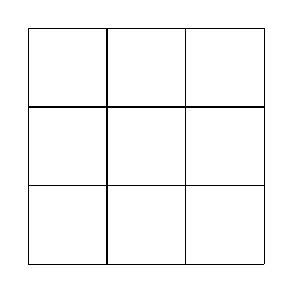
\begin{tikzpicture}
  \draw[] (0,0) grid (3,3);
\end{tikzpicture} & 

\begin{tikzpicture}
  \draw[] (0,0) grid (1,1);
\end{tikzpicture}  \vspace{10pt}\\
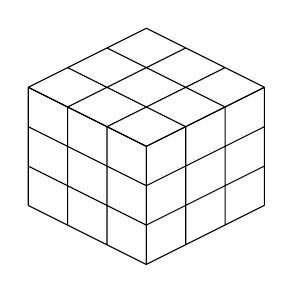
\begin{tikzpicture}[scale=0.5]
  \draw[yslant=-0.5] (0,0) grid (3,3);
  \draw[yslant=0.5] (3,-3) grid (6,0);
  \draw[yslant=0.5,xslant=-1] (3,0) grid (6,3);
\end{tikzpicture} & 

\begin{tikzpicture}[scale=0.5]
  \draw[yslant=-0.5] (0,0) grid (1,1);
  \draw[yslant=0.5] (1,-1) grid (2,0);
  \draw[yslant=0.5,xslant=-1] (1,0) grid (2,1);
\end{tikzpicture}
\end{tabular}
\end{document}